\section{Testing} %chen+tom
   
   Tests were performed in order to profile the code's performance and scalability. The unix \emph{time} command was 
   used to time the code runs, with `user' and `system' time being summed to find the total computation time.\newline{}
   
   The relationship between total computation time per cell and the number of cells was measured in order to quantify the overhead
   needed by the code (see Figure \ref{overhead}). We found that, below a grid size of $\sim$100 by 100, overhead became important, whereas at 
   larger grid sizes the computation time scaled linearly with the total number of cells. Any scaling worse than linear (such as 
   total computation time being proportional to the NumberOfCells$^{1.2}$ would be a huge (and unnecessary) inefficiency, especially with larger grids.\newline{}
   
   Some overhead is inevitable in any code, but the amount of effort put into simplifying a problem (such as creating arrays of neighbours)
   should depend on the expected size of the problem. Our code could probably have had less overhead, allowing it to run faster with smaller grid sizes,
   but this would likely led to it having a worse (linear) scaling with cell number.
   
   
   
   \section{Analysis} %tom+chen
   
   \begin{figure}[h]
   
   % GNUPLOT: LaTeX picture with Postscript
\begingroup
  \makeatletter
  \providecommand\color[2][]{%
    \GenericError{(gnuplot) \space\space\space\@spaces}{%
      Package color not loaded in conjunction with
      terminal option `colourtext'%
    }{See the gnuplot documentation for explanation.%
    }{Either use 'blacktext' in gnuplot or load the package
      color.sty in LaTeX.}%
    \renewcommand\color[2][]{}%
  }%
  \providecommand\includegraphics[2][]{%
    \GenericError{(gnuplot) \space\space\space\@spaces}{%
      Package graphicx or graphics not loaded%
    }{See the gnuplot documentation for explanation.%
    }{The gnuplot epslatex terminal needs graphicx.sty or graphics.sty.}%
    \renewcommand\includegraphics[2][]{}%
  }%
  \providecommand\rotatebox[2]{#2}%
  \@ifundefined{ifGPcolor}{%
    \newif\ifGPcolor
    \GPcolortrue
  }{}%
  \@ifundefined{ifGPblacktext}{%
    \newif\ifGPblacktext
    \GPblacktexttrue
  }{}%
  % define a \g@addto@macro without @ in the name:
  \let\gplgaddtomacro\g@addto@macro
  % define empty templates for all commands taking text:
  \gdef\gplbacktext{}%
  \gdef\gplfronttext{}%
  \makeatother
  \ifGPblacktext
    % no textcolor at all
    \def\colorrgb#1{}%
    \def\colorgray#1{}%
  \else
    % gray or color?
    \ifGPcolor
      \def\colorrgb#1{\color[rgb]{#1}}%
      \def\colorgray#1{\color[gray]{#1}}%
      \expandafter\def\csname LTw\endcsname{\color{white}}%
      \expandafter\def\csname LTb\endcsname{\color{black}}%
      \expandafter\def\csname LTa\endcsname{\color{black}}%
      \expandafter\def\csname LT0\endcsname{\color[rgb]{1,0,0}}%
      \expandafter\def\csname LT1\endcsname{\color[rgb]{0,1,0}}%
      \expandafter\def\csname LT2\endcsname{\color[rgb]{0,0,1}}%
      \expandafter\def\csname LT3\endcsname{\color[rgb]{1,0,1}}%
      \expandafter\def\csname LT4\endcsname{\color[rgb]{0,1,1}}%
      \expandafter\def\csname LT5\endcsname{\color[rgb]{1,1,0}}%
      \expandafter\def\csname LT6\endcsname{\color[rgb]{0,0,0}}%
      \expandafter\def\csname LT7\endcsname{\color[rgb]{1,0.3,0}}%
      \expandafter\def\csname LT8\endcsname{\color[rgb]{0.5,0.5,0.5}}%
    \else
      % gray
      \def\colorrgb#1{\color{black}}%
      \def\colorgray#1{\color[gray]{#1}}%
      \expandafter\def\csname LTw\endcsname{\color{white}}%
      \expandafter\def\csname LTb\endcsname{\color{black}}%
      \expandafter\def\csname LTa\endcsname{\color{black}}%
      \expandafter\def\csname LT0\endcsname{\color{black}}%
      \expandafter\def\csname LT1\endcsname{\color{black}}%
      \expandafter\def\csname LT2\endcsname{\color{black}}%
      \expandafter\def\csname LT3\endcsname{\color{black}}%
      \expandafter\def\csname LT4\endcsname{\color{black}}%
      \expandafter\def\csname LT5\endcsname{\color{black}}%
      \expandafter\def\csname LT6\endcsname{\color{black}}%
      \expandafter\def\csname LT7\endcsname{\color{black}}%
      \expandafter\def\csname LT8\endcsname{\color{black}}%
    \fi
  \fi
  \setlength{\unitlength}{0.0500bp}%
  \begin{picture}(7200.00,4536.00)%
    \gplgaddtomacro\gplbacktext{%
      \csname LTb\endcsname%
      \put(1100,640){\makebox(0,0)[r]{\strut{}-3.5}}%
      \put(1100,1111){\makebox(0,0)[r]{\strut{}-3.0}}%
      \put(1100,1582){\makebox(0,0)[r]{\strut{}-2.5}}%
      \put(1100,2053){\makebox(0,0)[r]{\strut{}-2.0}}%
      \put(1100,2523){\makebox(0,0)[r]{\strut{}-1.5}}%
      \put(1100,2994){\makebox(0,0)[r]{\strut{}-1.0}}%
      \put(1100,3465){\makebox(0,0)[r]{\strut{}-0.5}}%
      \put(1100,3936){\makebox(0,0)[r]{\strut{} 0.0}}%
      \put(1220,440){\makebox(0,0){\strut{} 0}}%
      \put(2167,440){\makebox(0,0){\strut{} 1}}%
      \put(3113,440){\makebox(0,0){\strut{} 2}}%
      \put(4060,440){\makebox(0,0){\strut{} 3}}%
      \put(5007,440){\makebox(0,0){\strut{} 4}}%
      \put(5953,440){\makebox(0,0){\strut{} 5}}%
      \put(6900,440){\makebox(0,0){\strut{} 6}}%
      \put(400,2288){\rotatebox{90}{\makebox(0,0){\strut{}log$_{10}$ Time/Cell [s]}}}%
      \put(4060,140){\makebox(0,0){\strut{}log$_{10}$ Number of Cells}}%
      \put(4060,4236){\makebox(0,0){\strut{}Run Time/Number of Cells vs. Number of Cells}}%
    }%
    \gplgaddtomacro\gplfronttext{%
      \csname LTb\endcsname%
      \put(5997,3773){\makebox(0,0)[r]{\strut{}Run Time/Number of Cells}}%
    }%
    \gplbacktext
    \put(0,0){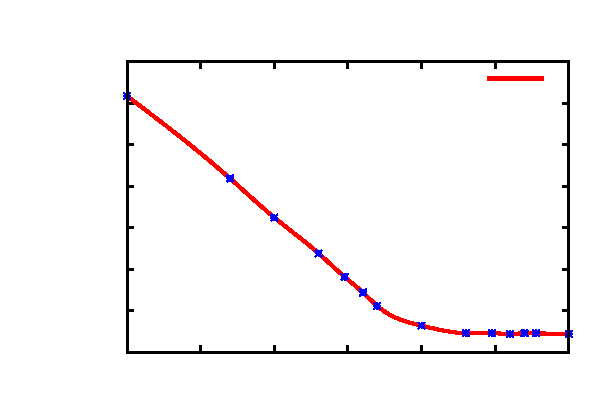
\includegraphics{figs/overhead}}%
    \gplfronttext
  \end{picture}%
\endgroup

   \caption{\label{overhead}This is a graph of total time spent on each cell, which shows that overheads such as array initialisation
   and output (i.e. things not directly involved in the simulation) take up a significant fraction of computation
   time with grids smaller than $\sim$100 by 100.}
   \end{figure}

  



